%!TEX root = ../../main.tex

\toggletrue{image}
\toggletrue{imagehover}
\chapterimage{dating_service}
\chapterimagetitle{\uppercase{Dating Service}}
\chapterimageurl{https://xkcd.com/120/}
\chapterimagehover{I don't understand why people are so disingenuous! I just want someone to walk with!}

\chapter{Dienste}
\label{chapter-dienste}

Das \ac{WWW} und das Internet werden im Alltag oft als Synonyme benutzt. Es heisst unter anderem in Nachrichtensendungen oft, dass man weitere Informationen im Internet unter der Adresse \url{www.tagesschau.ch} bzw. \url{www.tagesschau.de} findet. Korrekt müsste es eigentlich heissen, dass man weitere Informationen im \ac{WWW} findet, falls die Nachrichtensendung auf Ihren Webauftritt verweisen möchte. Wir möchten in diesem Kapitel die beiden Begriffe genauer unter die Lupe nehmen und korrekt einordnen. Die Lernziele lauten:

\newcommand{\diensteLernziele}{
\protect\begin{todolist}
\item Sie erklären den Unterschied zwischen einem Computernetzwerk und einem Dienst.
\item Sie erklären, was man unter einem Internetdienst versteht.
\item Sie nennen und beschreiben mehrere Internetdienste (z.B. das \ac{WWW}).
\end{todolist}
}

\lernziel{\autoref{chapter-dienste}, \nameref{chapter-dienste}}{\protect\diensteLernziele}

\diensteLernziele

%https://lehrerfortbildung-bw.de/u_matnatech/informatik/gym/bp2016/fb1/3_rechner_netze/1_hintergrund/3_kommunikation/02_run_hintergrund_netzwerke.pdf

\section{Was ist ein Dienst?}

Bisher haben wir das Internet als Infrastruktur für den Datenaustausch zwischen Computern kennengelernt. Eine Person kann das Internet aber so noch nicht wirklich benutzen. Es benötigt Programme, welche im Internet zur Verfügung stehen und benutzt werden können.

\begin{definition}[Dienst (eng. service)]
Ein Netzwerkdienst (kurz Dienst) ist ein Programm, welches auf einem oder mehreren Computern im Netzwerk ausgeführt wird. Das Programm ist über das Netzwerk erreichbar und bietet den Benutzern eine Funktion an.
\end{definition}

Dienste sind meist unter einem Namen bekannt und besitzen eine spezielle Funktion.

\begin{example}[Druckservice]
Neben den Computer können auch Drucker am Netzwerk beteiligt sein (Netzwerkdrucker). Ein typischer Netzwerkdienst ist das Drucken über das Netzwerk. Wir können von einem beliebigen Computer einen Druckauftrag über das Netzwerk starten und an einem beliebigen Drucker auslösen. Für das Drucken im Netzwerk ist ein Programm auf einem Computer installiert. Der Computer und das Programm sind ständig im Netzwerk erreichbar und können Druckaufträge verwalten. Diese Funktionalität stellt einen Netzwerkdienst dar.
\end{example}

%https://www.uni-giessen.de/fbz/svc/hrz/org/mitarb/abt/3/zms/schulung/webtechniken/internet

\begin{important}[Netzwerk $\neq$ Dienst]
Das Netzwerk ist die technische Infrastruktur (Leitungen, Computer, Router, Datenübertragung etc.), die von einem Dienst genutzt wird, um eine Funktion anzubieten.
\end{important}

Viele Dienste sind Ihnen vielleicht nicht explizit bewusst, aber aus Ihrem Alltag nicht mehr wegzudenken. Diese bekannten Dienste benutzen das Internet als Infrastruktur.

\begin{definition}[Internetdienst (eng. Internet service)]
Dienste, welche das Internet als Infrastruktur benutzen, werden Internetdienste genannt.
\end{definition}

\begin{example}
Es gibt zahlreiche Internetdienste. Wir nennen hier ein paar prominente Vertreter. Folgende Internetdienste nutzt der Benutzer mithilfe eines Programms direkt:

\begin{itemize}
	\item Das \textbf{\ac{WWW}} ist wohl der bekannteste Internetdienst. Es ist ein Informationsangebot. Ein Computerprogramm, der sogenannte Webserver, stellt Webseiten zur Verfügung. Ein Browser wird dann dazu benutzt, um die Webseiten vom Webserver anzufragen.
	\item Der Versand von \textbf{E-Mails} ist ein Internetdienst. Ein Sender schickt über das Internet eine E-Mail an einen Empfänger.
	\item \textbf{Online-Multiplayer-Computerspiele} (z.B. World of Warcraft) verbinden sich, um miteinander/gegeneinander zu spielen.
	\item \textbf{Instant Messaging} (z.B. WhatsApp) ist ein Internetdienst zum Nachrichtenversand.
	\item Das Abrufen von Musik und Video erfolgt über \textbf{Streamingdienste} im Internet.
\end{itemize}

Es gibt auch Internetdienste, welche nicht direkt durch eine Person genutzt werden. Es sind Computerprogramme, welche meist selbstständig die Dienste in Anspruch nehmen (sogenannten \ac{M2M}-Kommunikation). Einige Beispiele sind:

\begin{itemize}
	\item Das automatische Einklinken eines Computers in ein Netzwerk ohne eine Konfiguration des Benutzers wird über einen \ac{DHCP}-Service realisiert.
	\item Zur Synchronisation der Uhrzeit bietet der \textbf{Timedienst} eine hochgenaue Uhrzeit an. Die Uhrzeit wird durch eine \say{Referenzuhr} ermittelt und an die Computer verteilt.
	\item Damit Menschen die Webseiten im \ac{WWW} durch die relativ einfache Eingabe von einer Domain abrufen können (z.B. \url{webdev.ginf.ch}) existiert der \ac{DNS}-Service. Dieser übersetzt die Domains in die \say{echten} Adressen der Computer im Netzwerk (sogenannte \ac{IP}-Adressen).
\end{itemize}

\end{example}

\begin{figure}[htb]
\centering
\caption*{\uppercase{Messaging Systems} (\url{https://xkcd.com/2365/})}
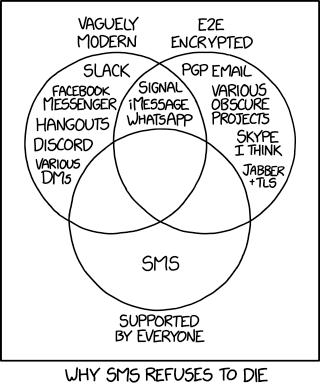
\includegraphics[scale=0.39]{messaging_systems}
\caption*{SMS is just the worst, but I'm having trouble convincing people to adopt my preferred system, TLS IRC with a local server and a patched DOSBox gateway running in my mobile browser.}
\label{figure-xkcd-2365}
\end{figure}